\documentclass[12pt]{report}
\usepackage{listings}
\usepackage{amsmath}
\usepackage[pdftex]{graphicx}
\usepackage{fancyvrb}
\usepackage{chapterbib}
\usepackage{hyperref}

\pdfcompresslevel=9
\DeclareGraphicsExtensions{{.png},{.pdf},{.jpg},{jpeg}}
\graphicspath{ {../figures/}}
\usepackage{color}

\begin{document}


\title{Uintah Application Development}

\author{John Schmidt}

\maketitle

\tableofcontents

\newpage


\chapter{Overview of the Uintah Framework}

The Uintah Computational Framework, i.e. \textbf{Uintah} consists of a
set of software components and libraries that facilitate the solution
of Partial Differential Equations (PDEs) on Structured AMR (SAMR)
grids using hundreds to thousands of processors.

One of the challenges in designing a parallel, component-based
multi-physics application is determining how to efficiently decompose
the problem domain. Components, by definition, make local
decisions. Yet parallel efficiency is only obtained through a globally
optimal domain decomposition and scheduling of computational
tasks. Typical techniques include allocating disjoint sets of
processing resources to each component, or defining a single domain
decomposition that is a compromise between the ideal load balance of
multiple components. However, neither of these techniques will achieve
maximum efficiency for complex multi-physics problems.

Uintah uses a non-traditional approach to achieving parallelism,
employing an abstract taskgraph representation to describe computation
and communication. The taskgraph is an explicit representation of the
computation and communication that occur in the coarse of a single
iteration of the simulation (typically a timestep or nonlinear solver
iteration) see figure~\ref{fig:TaskGraph}. Uintah components delegate
decisions about parallelism to a scheduler component, using variable
dependencies to describe communication patterns and characterizing
computational workloads to facilitate a global resource
optimization. The taskgraph representation has a number of advantages,
including efficient fine-grained coupling of multi-physics components,
flexible load balancing mechanisms and a separation of application
concerns from parallelism concerns. However, it creates a challenge
for scalability which we overcome by creating an implicit definition
of this graph and representing it in a distributed fashion.
\begin{figure}
  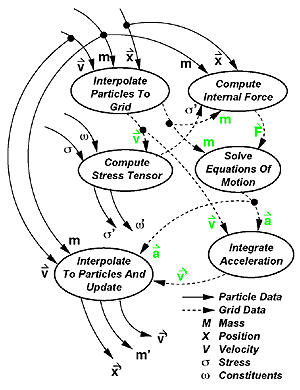
\includegraphics[scale=1]{Taskgraph-diagram.png}
  \caption{Example Task Graph}
  \label{fig:TaskGraph}
\end{figure}


The primary advantage of a component-based approach is that it
facilitates the separate development of simulation algorithms, models,
and infrastructure. Components of the simulation can evolve
independently. The component-based architecture allows pieces of the
system to be implemented in a rudimentary form at first and then
evolve as the technologies mature. Most importantly, Uintah allows the
aspects of parallelism (schedulers, load-balancers, parallel
input/output, and so forth) to evolve independently of the simulation
components. Furthermore, components enable replacement of computation
pieces without complex decision logic in the code itself.

\section{Scheduler}

The Scheduler in Uintah is responsible for determining the order of
tasks and ensuring that the correct inter-processor data is made
available when necessary. Each software component passes a set of
tasks to the scheduler. Each task is responsible for computing some
subset of variables, and may require previously computed variables,
possibly from different processors. The scheduler will then compile
this task information into a task graph, and the task graph will
contain a sorted order of tasks, along with any information necessary
to perform inter-process communication via MPI. Then, when the
scheduler is executed, the tasks will execute in the pre-determined
order.

\subsection{needRecompile()}

%% Not sure where this information really should go, but wanted to
%% save it for posterity...

Each component has a needRecompile() function that is called once per
timestep.  If, for whatever reason, a Component determines that the
list of tasks it had previously scheduled is no longer valid, then the
Component must return 'true' when its needRecompile() function is
called.  This will cause the scheduler to rebuild the task graph (by
asking each component to re-specify tasks).  Note, rebuilding the
taskgraph is a relatively expensive operation, so only should be done
if necessary.

\section{Tasks}

A task contains two essential components: a pointer to a function
that performs the actual computations, and the data inputs and
outputs, i.e. the data dependencies required by the function.  When a
task requests a previously computed variable from the data warehouse,
the number of ghost cells are also specified.  The Unitah framework
uses the ghost cell information to excecute inter-process
communication to retrieve the necessary ghost cell data.

An example of a task description is presented showing the essential
features that are commonly used by the application developer when
implementing an algorithm within the Uintah framework.  The task
component is assigned a name and in this particular example, it is
called \texttt{taskexample} and a function pointer,
\texttt{\&Example::taskexample}.  Following the instantiation of the
task itself, the dependency information is assigned to the tasks.  In
the following example, the task requires data from the previous
timestep (\texttt{Task::OldDW}) associated with the name
variable1\_label and requires one ghost node
(\texttt{Ghost::AroundNodes,1}) level of information which will be
retrieved from another processor via MPI.  In addition, the task will
compute two new pieces of data each associated with different
variables, i.e. \texttt{variable1\_label}, and
\texttt{variable2\_label}.  Finally, the task is added to the scheduler
component with specifications about what patches and materials are
associated with the actual computation.

\begin{Verbatim}[fontsize=\footnotesize]

Task* task = scinew Task("Example::taskexample",this,
                         &Example::taskexample);
task->requires(Task::OldDW, variable1_label, Ghost::AroundNodes, 1);
task->computes(variable1_label);
task->computes(variable2_label);
sched->addTask(task, level->eachPatch(), sharedState_->allMaterials());

\end{Verbatim}

For more complex problems involving multiple materials and
multi-physics calculations, a subset of the materials may only be used
in the calculation of particular tasks.  The Uintah framework allows
for the independent scheduling and computation of multi-material
within a multi-physics calculation.

\section{Tasks and Scheduler Description -- Programmer Interface}

\subsection{Simulation Component Class Description}

Each Uintah component can be described as a C++ class that is derived
from two other classes: \textbf{UintahParallelComponent} and a
\textbf{SimulationInterface}. The new derived class must provide the
following virtual methods: \texttt{problemSetup},
\texttt{scheduleInitialize}, \texttt{scheduleComputeStableTimestep},
and \texttt{scheduleTimeAdvance}.  Here is an example of the typical
*.h file that needs to be created for a new component.

\begin{Verbatim}[fontsize=\footnotesize]


class Example : public UintahParallelComponent, public SimulationInterface {
  public:

    virtual void problemSetup(const ProblemSpecP& params, 
                              const ProblemSpecP& restart_prob_spec, 
                              GridP& grid, SimulationStateP&);

    virtual void scheduleInitialize(const LevelP& level,SchedulerP& sched);
                                    
    virtual void scheduleComputeStableTimestep(const LevelP& level, 
                                               SchedulerP&);
                                               
    virtual void scheduleTimeAdvance(const LevelP& level, SchedulerP&);

   private:
    Example(const ProcessorGroup* myworld);
    virtual ~Example();


    void initialize(const ProcessorGroup*,
                    const PatchSubset* patches, 
                    const MaterialSubset* matls,
                    DataWarehouse* old_dw, 
                    DataWarehouse* new_dw);
                    
                    
    void computeStableTimestep(const ProcessorGroup*,
                               const PatchSubset* patches,
                               const MaterialSubset* matls,
                               DataWarehouse* old_dw,
                               DataWarehouse* new_dw);
                               
    void timeAdvance(const ProcessorGroup*,
                     const PatchSubset* patches,
                     const MaterialSubset* matls,
                     DataWarehouse* old_dw,
                     DataWarehouse* new_dw);

}


\end{Verbatim}


Each new component inherits from the classes
\textbf{UintahParrallelComponent} and \textbf{SimulationInterface}.
The component overrides default implementations of various methods.
The above methods are the essential functions that a new component
must implement.  Additional methods to do AMR will be described as
more complex examples are presented.

The roles of each of the scheduling methods are described below.  Each
scheduling method, i.e. \texttt{scheduleInitialize},
\texttt{scheduleComputeStableTimestep}, and
\texttt{scheduleTimeAdvance} describe

\subsubsection{ProblemSetup}



The purpose of this method is to read a problem specification which
requires a minimum of information about the grid used, time
information, i.e. time step size, length of time for simulation, etc,
and where and what data is actually saved.  Depending on the problem
that is solved, the input file can be rather complex, and this method
would evolve to establish any and all parameters needed to initially
setup the problem.

\subsubsection{ScheduleInitialize}

The purpose of this method is to initialize the grid data with values
read in from the problemSetup and to define what variables are
actually computed in the TimeAdvance stage of the simulation.  A task
is defined which references a function pointer called
\texttt{initialize}.

\subsubsection{ScheduleComputeStableTimestep}

The purpose of this method is to compute the next timestep in the
simulation.  A task is defined which references a function pointer
called \texttt{computeStableTimestep}.

\subsubsection{ScheduleTimeAdvance}

The purpose of this method is to schedule the actual algorithmic
implementation.  For simple algorithms, there is only one task defined
with a minimal set of data dependencies specified.  However, for more
complicated algorithms, the best way to schedule the algorithm is to
break it down into individual tasks.  Each task of the algorithm will
have its own data dependencies and function pointers that reference
individual computational methods.

\subsection{Data Storage Concepts}

During the course of the simulation, data is computed and stored in a
data structure called the DataWarehouse.  Data that is from a previous
timestep is stored in the Old DataWarehouse, called \texttt{OldDW},
and data that is computed in current timestep is stored in the New
DataWarehouse, called \texttt{NewDW}.  At the end of the timestep,
current timestep data is moved to the old data warehouse for the next
timestep in the simulation.

\chapter{Examples}


This chapter will describe a set of example problems showing various
stages of algorithm complexity and how the Uintah framework is used to
solve the discretized form of the solutions.  Emphasis will not be on
the most efficient or fast algorithms, but intead will demonstrate
straightforward implementations of well known algorithms within the
Uintah Framework.  Several examples will be given that show an
increasing level of complexity that will serve as a guide to others
interested in implmenting structured AMR algorithms for PDEs.

All examples described are found in the directory
\emph{SCIRun/src/Packages/Uintah/CCA/Components/Examples}

\section{Poisson1}

Poisson1 is solves Poisson's equation on a grid using Jacobi
iteration.  Since this is not a time dependent problem and Uintah is
fundamentally designed for time dependent problems, each Jacobi
iteration is considered to be a timestep.  The timestep specified and
computed is a fixed value obtained from the input file and has no
bearing on the actual computation.

The following equation is discretized and solved using an iterative
method. Each timestep is one iteration. At the end of the timestep, we
the residual is computed showing the convergence of the solution and
the next iteration is computed until.

The following shows a simplified form of the Poisson1 of the .h and
.cc files found in the Examples directory.  The argument list for some
of the methods are eliminated for readibility purposes.  Please refer
to the actual source for a complete description of the arguments
required for each method.

\begin{Verbatim}[fontsize=\footnotesize]
class Poisson1 : public UintahParallelComponent, public SimulationInterface {
  public:
    Poisson1(const ProcessorGroup* myworld);
    virtual ~Poisson1();

    virtual void problemSetup(const ProblemSpecP& params,
                              const ProblemSpecP& restart_prob_spec,
                              GridP& grid, SimulationStateP&);
    virtual void scheduleInitialize(const LevelP& level,SchedulerP& sched);

    virtual void scheduleComputeStableTimestep(const LevelP& level,SchedulerP&);

    virtual void scheduleTimeAdvance(const LevelP& level,SchedulerP&);

  private:
    void initialize(const ProcessorGroup*, const PatchSubset* patches,
                    const MaterialSubset* matls, DataWarehouse* old_dw,
                    DataWarehouse* new_dw);

    void computeStableTimestep(const ProcessorGroup*,const PatchSubset* patches,
                               const MaterialSubset* matls,DataWarehouse* old_dw,
                               DataWarehouse* new_dw);


    void timeAdvance(const ProcessorGroup,const PatchSubset* patches,
                     const MaterialSubset* matls,DataWarehouse* old_dw,
                     DataWarehouse* new_dw);

    SimulationStateP sharedState_;
    double delt_;
    const VarLabel* phi_label;
    const VarLabel* residual_label;
    SimpleMaterial* mymat_;

    Poisson1(const Poisson1&);
    Poisson1& operator=(const Poisson1&);
};
\end{Verbatim}

The private methods and data shown are the functions that are function
pointers referred to in the task descriptions.  The \texttt{VarLabel}
data type stores the names of the various data that can be referenced
uniquely by the data warehouse.  The \texttt{SimulationStateP} data
type is essentially a global variable that stores information about
the materials that are needed by other internal Uintah framework
components.  \texttt{SimpleMaterial} is a data type that refers to the
material properties.

Within each schedule function, i.e. \texttt{sheduleInitialize},
\texttt{scheduleComputeStableTimestep}, and
\texttt{scheduleTimeAdvance}, a task is specified that has a function
pointer associated with it.  The function pointers point to the actual
implementation of the specific task and have a different argument list
than the associated schedule method.

The typical task implementation, i.e. \texttt{timeAdvance()} contains
the following arguments: \texttt{ProcessorGroup},
\texttt{PatchSubset}, \texttt{MaterialSubset}, and two
\texttt{DataWarehouse} objects.  The purpose of the
\texttt{ProcessorGroup} is to hold various MPI information such as the
\texttt{MPI\_Communicator}, the rank of the process and the number of
processes that are actually being used.

\subsection{Description of Scheduling Functions}

The actual implementation with descriptions are presented following
the code snippets.

\begin{Verbatim}[fontsize=\footnotesize]
Poisson1::Poisson1(const ProcessorGroup* myworld)
  : UintahParallelComponent(myworld)
{
  phi_label = VarLabel::create("phi", 
                               NCVariable<double>::getTypeDescription());
  residual_label = VarLabel::create("residual", 
                                    sum_vartype::getTypeDescription());

}

Poisson1::~Poisson1()
{
  VarLabel::destroy(phi_label);
  VarLabel::destroy(residual_label);
}

\end{Verbatim}

Typical constructor and destructor for simple examples where the data
label names (\texttt{phi} and \texttt{residual}) are created for data
wharehouse storage and retrieval.

\begin{Verbatim}[fontsize=\footnotesize]
void Poisson1::problemSetup(const ProblemSpecP& params,
                            const ProblemSpecP& restart_prob_spec,
                            GridP& /*grid*/,
                            SimulationStateP& sharedState)
{
  sharedState_ = sharedState;
  ProblemSpecP poisson = params->findBlock("Poisson");

  poisson->require("delt", delt_);

  mymat_ = scinew SimpleMaterial();

  sharedState->registerSimpleMaterial(mymat_);
}
\end{Verbatim}

The \texttt{problemSetup} is based in a xml description of the input
file.  The input file is parsed and the delt tag is set.  The
\texttt{sharedState} is assigned and is used to register a material
and store it for later use by the Uintah internals.

\begin{Verbatim}[fontsize=\footnotesize]
void Poisson1::scheduleInitialize(const LevelP& level,
                                  SchedulerP& sched)
{
  Task* task = scinew Task("Poisson1::initialize",
                     this, &Poisson1::initialize);

  task->computes(phi_label);
  task->computes(residual_label);
  sched->addTask(task, level->eachPatch(), sharedState_->allMaterials());
}
\end{Verbatim}

A task is defined which contains a name and a function pointer,
i.e. \texttt{initialize} which is described later in Poisson1.cc The
task defines two variables that are computed in the
\texttt{initialize} function, \texttt{phi} and \texttt{residual}.  The
task is then added to the scheduler.  This task is only computed once
at the beginning of the simulation.

\begin{Verbatim}[fontsize=\footnotesize]
void Poisson1::scheduleComputeStableTimestep(const LevelP& level,
                                             SchedulerP& sched)
{
  Task* task = scinew Task("Poisson1::computeStableTimestep",
                     this, &Poisson1::computeStableTimestep);

  task->requires(Task::NewDW, residual_label);
  task->computes(sharedState_->get_delt_label());
  sched->addTask(task, level->eachPatch(), sharedState_->allMaterials());
}

\end{Verbatim}

A task is defined for the computing the stable timestep and uses the
function pointer, \texttt{computeStableTimestep} defined later in
Poisson1.cc.  This requires data from the New DataWarehouse, and the
next timestep size is computed and stored.

\begin{Verbatim}[fontsize=\footnotesize]
void
Poisson1::scheduleTimeAdvance( const LevelP& level,
                               SchedulerP& sched)
{
  Task* task = scinew Task("Poisson1::timeAdvance",
                     this, &Poisson1::timeAdvance);

  task->requires(Task::OldDW, phi_label, Ghost::AroundNodes, 1);
  task->computes(phi_label);
  task->computes(residual_label);
  sched->addTask(task, level->eachPatch(), sharedState_->allMaterials());
}
\end{Verbatim}

The \texttt{timeAdvance} function is the main function that describes
the computational algorithm.  For simple examples, the entire
algorithm is usually defined by one task with a small set of data
dependencies.  However, for more complicated algorithms, it is best to
break the algorithm down into a set of tasks with each task describing
its own set of data dependencies.

For this example, a single task is described and the
\texttt{timeAdvance} function pointer is specified.  Data from the
previous timestep (\texttt{OldDW}) is required for the current
timestep.  For a simple seven (7) point stencil, only one level of
ghost cells is required.  The algorithm is set up for nodal values,
the ghost cells are specified by the the \texttt{Ghost::AroundNodes}
syntax.  The task computes both the new data values for phi and a
residual.

\subsection{Description of Computational Functions}

\begin{Verbatim}[fontsize=\footnotesize]

void Poisson1::computeStableTimestep(const ProcessorGroup* pg,
                                     const PatchSubset* /*patches*/,
                                     const MaterialSubset* /*matls*/,
                                     DataWarehouse*,
                                     DataWarehouse* new_dw)
{
  if(pg->myrank() == 0){
    sum_vartype residual;
    new_dw->get(residual, residual_label);
    cerr << "Residual=" << residual << '\n';
  }
  new_dw->put(delt_vartype(delt_), sharedState_->get_delt_label());
}

\end{Verbatim}

In this particular example, no timestep is actually computed, instead
the original timestep specified in the input file is used and stored
in the data warehouse (\texttt{new\_dw->put(delt\_vartype(delt\_),
  sharedState\_\->get\_delt\_label())}).  The residual computed in the
main \texttt{timeAdvance} function is retrieved from the data
warehouse and printed out to standard error for only the processor
with a rank of 0.

\begin{Verbatim}[fontsize=\footnotesize]
void Poisson1::initialize(const ProcessorGroup*,
                          const PatchSubset* patches,
                          const MaterialSubset* matls,
                          DataWarehouse* /*old_dw*/, DataWarehouse* new_dw)
{
  int matl = 0;
  for(int p=0;p<patches->size();p++){
    const Patch* patch = patches->get(p);

\end{Verbatim}

The node centered variable (\texttt{NCVariable<double> phi}) has space
reserved in the DataWarehouse for the given patch and the given
material (\texttt{int matl = 0;}).  The \texttt{phi} variable is
initialized to 0 for every grid node on the patch.

\begin{Verbatim}[fontsize=\footnotesize]
    NCVariable<double> phi;
    new_dw->allocateAndPut(phi, phi_label, matl, patch);
    phi.initialize(0.);
\end{Verbatim}

The boundary faces on the xminus face of the computational domain are
specified and set to a value of 1.  All other boundary values are set
to a value of 0 as well as the internal nodes via the
\texttt{phi.initialize(0.)} construct.  Uintah provides helper
functions for determining which nodes are on the boundaries.  In
addition, there are convenient looping constructs such as
\texttt{NodeIterator} that alleviate the need to specify triply nested
loops for visiting each node in the domain.

\begin{Verbatim}[fontsize=\footnotesize]
    if(patch->getBCType(Patch::xminus) != Patch::Neighbor){
       IntVector l,h;
       patch->getFaceNodes(Patch::xminus, 0, l, h);

      for(NodeIterator iter(l,h); !iter.done(); iter++){
         phi[*iter]=1;
      }
    }

    new_dw->put(sum_vartype(-1), residual_label);
  }
}

\end{Verbatim}

The initial residual value of -1 is stored at the beginning of the
simulation.

The main computational algorithm is defined in the
\texttt{timeAdvance} function.  The overall algorithm is based on a
simple Jacobi iteration step.

\begin{Verbatim}[fontsize=\footnotesize]
void Poisson1::timeAdvance(const ProcessorGroup*,
                           const PatchSubset* patches,
                           const MaterialSubset* matls,
                           DataWarehouse* old_dw,
                           DataWarehouse* new_dw)
{
  int matl = 0;
  for(int p=0;p<patches->size();p++){
    const Patch* patch = patches->get(p);
    constNCVariable<double> phi;

\end{Verbatim}

Data from the previous timestep is retrieved from the data warehouse
and copied to the current timestep's phi variable (\texttt{newphi}).

\begin{Verbatim}[fontsize=\footnotesize]

    old_dw->get(phi, phi_label, matl, patch, Ghost::AroundNodes, 1);
    NCVariable<double> newphi;

    new_dw->allocateAndPut(newphi, phi_label, matl, patch);
    newphi.copyPatch(phi, newphi.getLowIndex(), newphi.getHighIndex());

\end{Verbatim}

The indices for the patch are obtained and altered depending on
whether or not the patch's internal boundaries are on the coincident
with the grid domain.  If the patch boundaries are the same as the
grid domain, the boundary values are not overwritten since the lower
and upper indices are modified to only specify internal nodal grid
points.


%%% The implementation of more sensible boundary condition
%%% specifications needs to be added here.

\begin{Verbatim}[fontsize=\footnotesize]

    double residual=0;
    IntVector l = patch->getNodeLowIndex__New();
    IntVector h = patch->getNodeHighIndex__New();

    l += IntVector(patch->getBCType(Patch::xminus) == Patch::Neighbor?0:1,
                   patch->getBCType(Patch::yminus) == Patch::Neighbor?0:1,
                   patch->getBCType(Patch::zminus) == Patch::Neighbor?0:1);
    h -= IntVector(patch->getBCType(Patch::xplus)  == Patch::Neighbor?0:1,
                   patch->getBCType(Patch::yplus)  == Patch::Neighbor?0:1,
                   patch->getBCType(Patch::zplus)  == Patch::Neighbor?0:1);

\end{Verbatim}

The Jacobi iteration step is applied at each internal grid node.  The
residual is computed based on the old and new values and stored as a
reduction variable (\texttt{sum\_vartype}) in the data warehouse.

\begin{Verbatim}[fontsize=\footnotesize]
    //__________________________________
    //  Stencil
    for(NodeIterator iter(l, h);!iter.done(); iter++){
      IntVector n = *iter;

      newphi[n]=(1./6)*(
        phi[n+IntVector(1,0,0)] + phi[n+IntVector(-1,0,0)] +
        phi[n+IntVector(0,1,0)] + phi[n+IntVector(0,-1,0)] +
        phi[n+IntVector(0,0,1)] + phi[n+IntVector(0,0,-1)]);

      double diff = newphi[n] - phi[n];
      residual += diff * diff;
    }
    new_dw->put(sum_vartype(residual), residual_label);
  }
}

\end{Verbatim}

The input file that is used to run this example is given below and is
given in
\emph{SCIRun/src/Packages/Uintah/StandAlone/inputs/Examples/poisson1.ups}.
Relevant sections of the input file that can be modified are found in
the \texttt{<Time>} section, and the \texttt{<Grid>} section,
specifically, the number of patches and the grid resolution.

\begin{Verbatim}[fontsize=\footnotesize]
<Uintah_specification>

  <Meta>
      <title>Poisson1 test</title>
  </Meta>

  <SimulationComponent>
       <type> poisson1 </type>
  </SimulationComponent>
  <!--__________________________________-->
  <Time>
    <maxTime>       1.0       </maxTime>
    <initTime>      0.0       </initTime>
    <delt_min>      0.00001   </delt_min>
    <delt_max>      1         </delt_max>
    <max_Timesteps> 100        </max_Timesteps>
    <timestep_multiplier>  1  </timestep_multiplier>
  </Time>

  <!--__________________________________-->
  <DataArchiver>
  <filebase>poisson.uda</filebase>
      <outputTimestepInterval>1</outputTimestepInterval>
      <save label = "phi"/>
      <save label = "residual"/>
      <checkpoint cycle = "2" timestepInterval = "1"/>
  </DataArchiver>


  <!--__________________________________-->
  <Poisson>
    <delt>.01</delt>
    <maxresidual>.01</maxresidual>
  </Poisson>


  <!--__________________________________-->
  <Grid>
    <Level>
      <Box label = "1">
         <lower>     [0,0,0]        </lower>
         <upper>     [1.0,1.0,1.0]  </upper>
         <resolution>[50,50,50]     </resolution>
         <patches>   [2,1,1]        </patches>
      </Box>
    </Level>
</Grid>

</Uintah_specification>

\end{Verbatim}


\subsubsection{Running the Poisson1 Example}

To run the poisson1.ups example, 
\begin{Verbatim}[fontsize=\footnotesize]

	cd ~/SCIRun/dbg/Packages/Uintah/StandAlone/
\end{Verbatim}

create a symbolic link to the inputs directory:
\begin{Verbatim}[fontsize=\footnotesize]
	ln -s ~/SCIRun/src/Packages/Uintah/StandAlone/inputs
\end{Verbatim}
For a single processor run type the following:
\begin{Verbatim}[fontsize=\footnotesize]
	sus inputs/Examples/poisson1.ups
\end{Verbatim}
For a two processor run, type the following:
\begin{Verbatim}[fontsize=\footnotesize]
	mpirun -np 2 sus -mpi inputs/Examples/poisson1.ups
\end{Verbatim}
Changing the number of patches in the poisson1.ups and the resolution,
enables you to run a more refined problem on more processors.

\textbf{ADVICE:} For non-AMR problems, it is advised to have at least
the same number of patches as processors.  You can always have more
patches than processors, but you cannot have fewer patches than
processors.


\section{Poisson2}

The next example also solves the Poisson's equation but instead of
iterating in time, the subscheduler feature iterates within a given
timestep, thus solving the problem in one timestep.  The use of the
subcheduler is important for implementing algorithms which solve
non-linear problems which require iterating on a solution for each
timestep.

The majority of the schedule and computational functions are similar
to the \emph{Poisson1} example and are not repeated.  Only the revised
code is presented with explanations about the new features of Uintah.

\begin{Verbatim}[fontsize=\footnotesize]

void Poisson2::scheduleTimeAdvance( const LevelP& level, SchedulerP& sched)
{
  Task* task = scinew Task("timeAdvance",
			this, &Poisson2::timeAdvance,
			level, sched.get_rep());
  task->hasSubScheduler();
  task->requires(Task::OldDW, phi_label, Ghost::AroundNodes, 1);
  task->computes(phi_label);
  LoadBalancer* lb = sched->getLoadBalancer();
  const PatchSet* perproc_patches = lb->getPerProcessorPatchSet(level);
  sched->addTask(task, perproc_patches, sharedState_->allMaterials());
}

\end{Verbatim}

Within this function, the task is specified with two additional
arguments, the level and the scheduler \texttt{sched.get\_rep()}.  The
task must also set the flag that a subscheduler will be used within
the scheduling of the various tasks.  Similar code to the
\textbf{Poisson1} example is used to specify what data is required and
computed during the actual task execution.  In addition, a
loadbalancer component is required to query the patch distribution for
each level of the grid.  The task is then added to the top level
scheduler with the requisite information, i.e. patches and materials.

The actual implementation of the \texttt{timeAdvance} function is also
different from the \textbf{Poisson1} example.  The code is specified
below with text explaining the use of the subscheduler.  The new
feature of the subscheduler shows the creation of a the
\texttt{iterate} task within the subscheduler.  This task will perform
the actual Jacobi iteration for a given timestep.

\begin{Verbatim}[fontsize=\footnotesize]
void Poisson2::timeAdvance(const ProcessorGroup* pg,
			const PatchSubset* patches,
			const MaterialSubset* matls,
			DataWarehouse* old_dw, DataWarehouse* new_dw,
			LevelP level, Scheduler* sched)
{

\end{Verbatim}

The subscheduler is instantiated and initialized. 

\begin{Verbatim}[fontsize=\footnotesize]
  SchedulerP subsched = sched->createSubScheduler();
  subsched->initialize();
  GridP grid = level->getGrid();
\end{Verbatim}

An \texttt{iterate} task is created and added to the subscheduler.
The typical computes and requires are specified for a 7 point stencil
used in Jacobi iteration scheme with one layer of ghost cells.  The
new task is added to the subscheduler.  A residual variable is only
computed within the subscheduler and not passed back to the main
scheduler.  This is in contrast to the \texttt{phi} variable which was
specified in \texttt{scheduleTimeAdvance} in the computes, as well as
being specified in the computes for the subscheduler.  Any variables
that are only computed and used in an iterative step of an algorithm
do not need to be added to the dependency specification for the top
level task.

\begin{Verbatim}[fontsize=\footnotesize]
  // Create the tasks
  Task* task = scinew Task("iterate",
			this, &Poisson2::iterate);
  task->requires(Task::OldDW, phi_label, Ghost::AroundNodes, 1);
  task->computes(phi_label);
  task->computes(residual_label);
  subsched->addTask(task, level->eachPatch(), sharedState_->allMaterials());
\end{Verbatim}

The subscheduler has its own data wharehouse that is separate from the
top level's scheduler's data warehouse.  This data warehouse must be
initialized and any data from the top level's data warehouse must be
passed to the subscheduler's version.  This data resides in the data
warehouse position \texttt{NewDW}.

\begin{Verbatim}[fontsize=\footnotesize]
  // Compile the scheduler
  subsched->advanceDataWarehouse(grid);
  subsched->compile();

  int count = 0;
  double residual;
  subsched->get_dw(1)->transferFrom(old_dw, phi_label, patches, matls);
\end{Verbatim}

Within each iteration, the following must occur for the subscheduler:
the data warehouse's new data must be moved to the \texttt{OldDW}
position, since any new values will be stored in \texttt{NewDW} and
the old values cannot be overwritten.  The \texttt{OldDW} is referred
to in the subscheduler via the \texttt{subsched->get\_dw(0)} and the
\texttt{NewDW} is referred to in the subscheduler via
\texttt{subsched->get\_dw(1)}.  Once the iteration is deemed to have
met the tolerance, the data from the subscheduler is transferred to
the scheduler's data warehouse.

\begin{Verbatim}[fontsize=\footnotesize]
  // Iterate
  do {
    subsched->advanceDataWarehouse(grid);
    subsched->get_dw(0)->setScrubbing(DataWarehouse::ScrubComplete);
    subsched->get_dw(1)->setScrubbing(DataWarehouse::ScrubNonPermanent);
    subsched->execute();    

    sum_vartype residual_var;
    subsched->get_dw(1)->get(residual_var, residual_label);
    residual = residual_var;

    if(pg->myrank() == 0)
      cerr << "Iteration " << count++ << ", residual=" << residual << '\n';
  } while(residual > maxresidual_);

  new_dw->transferFrom(subsched->get_dw(1), phi_label, patches, matls);
}

\end{Verbatim}

The iteration cycle is identical to \textbf{Poisson1}'s
\texttt{timeAdvance} algorithm using Jacobi iteration with a 7 point
stencil.  Refer to the discussion about the algorithm implementation
in the \textbf{Poisson1} description.

\begin{Verbatim}[fontsize=\footnotesize]
void Poisson2::iterate(const ProcessorGroup*,
		    const PatchSubset* patches,
		    const MaterialSubset* matls,
		    DataWarehouse* old_dw, DataWarehouse* new_dw)
{
  for(int p=0;p<patches->size();p++){
    const Patch* patch = patches->get(p);
    for(int m = 0;m<matls->size();m++){
      int matl = matls->get(m);
      constNCVariable<double> phi;
      old_dw->get(phi, phi_label, matl, patch, Ghost::AroundNodes, 1);
      NCVariable<double> newphi;
      new_dw->allocateAndPut(newphi, phi_label, matl, patch);
      newphi.copyPatch(phi, newphi.getLow(), newphi.getHigh());
      double residual=0;
      IntVector l = patch->getNodeLowIndex__New();
      IntVector h = patch->getNodeHighIndex__New(); 
      l += IntVector(patch->getBCType(Patch::xminus) == Patch::Neighbor?0:1,
		  patch->getBCType(Patch::yminus) == Patch::Neighbor?0:1,
		  patch->getBCType(Patch::zminus) == Patch::Neighbor?0:1);
      h -= IntVector(patch->getBCType(Patch::xplus) == Patch::Neighbor?0:1,
		  patch->getBCType(Patch::yplus) == Patch::Neighbor?0:1,
		  patch->getBCType(Patch::zplus) == Patch::Neighbor?0:1);
      for(NodeIterator iter(l, h);!iter.done(); iter++){
	newphi[*iter]=(1./6)*(
	phi[*iter+IntVector(1,0,0)]+phi[*iter+IntVector(-1,0,0)]+
	phi[*iter+IntVector(0,1,0)]+phi[*iter+IntVector(0,-1,0)]+
	phi[*iter+IntVector(0,0,1)]+phi[*iter+IntVector(0,0,-1)]);
	double diff = newphi[*iter]-phi[*iter];
	residual += diff*diff;
      }
      new_dw->put(sum_vartype(residual), residual_label);
    }
  }
}

\end{Verbatim}

The input file
\emph{~/SCIRun/src/Packages/Uintah/StandAlone/inputs/Examples/poisson2.ups}
is very similar to the \emph{poisson1.ups} file shown above.  The only
additional tag that is used is the \texttt{<maxresidual>} specifying
the tolerance within the iteration performed in the subscheduler.

To run the poisson2 input file execute the following in the
\emph{~/SCIRun/dbg/Packages/Uintah/StandAlone} directory:

\begin{Verbatim}[fontsize=\footnotesize]
	sus inputs/Examples/poisson2.ups

\end{Verbatim}


\section{Burger}

In this example, the inviscid Burger's equation is solved in three dimensions:
\begin{Verbatim}[fontsize=\footnotesize]
	du/dt = -u du/dx  
\end{Verbatim}

with the following initial conditions:

\begin{Verbatim}[fontsize=\footnotesize]
	u = sin(pi x) + sin(2pi y) + sin(3pi z)
\end{Verbatim}

using Euler's method to advance in time.  The majority of the code is
very similar to the Poisson1 example code with the differences shown
below.

The initialization of the grid values for the unknown variable, u, is
done at every grid node using the NodeIterator construct.  The x,y,z
values for a given grid node is determined using the function,
\texttt{patch->getNodePosition(n)}, where n is the nodal index in
i,j,k space.

\begin{Verbatim}[fontsize=\footnotesize]
void Burger::initialize(const ProcessorGroup*,
                        const PatchSubset* patches,
                        const MaterialSubset* matls,
                        DataWarehouse*, 
                        DataWarehouse* new_dw)
{
  int matl = 0;
  for(int p=0;p<patches->size();p++){
    const Patch* patch = patches->get(p);

    NCVariable<double> u;
    new_dw->allocateAndPut(u, u_label, matl, patch);

    //Initialize
    // u = sin( pi*x ) + sin( pi*2*y ) + sin(pi*3z )
    IntVector l = patch->getNodeLowIndex__New();
    IntVector h = patch->getNodeHighIndex__New();
    
    for( NodeIterator iter=patch->getNodeIterator__New(); !iter.done(); iter++ ){
      IntVector n = *iter;
      Point p = patch->nodePosition(n);
      u[n] = sin( p.x() * 3.14159265358 ) + sin( p.y() * 2*3.14159265358)  +  sin( p.z() * 3*3.14159265358);
    }
  }
}

\end{Verbatim}

The \texttt{timeAdvance} function is quite similar to the Poisson1's
\texttt{timeAdvance} routine.  The relavant differences are only
shown.

\begin{Verbatim}[fontsize=\footnotesize]
void Burger::timeAdvance(const ProcessorGroup*,
                         const PatchSubset* patches,
                         const MaterialSubset* matls,
                         DataWarehouse* old_dw, 
                         DataWarehouse* new_dw)
{
  int matl = 0;
  //Loop for all patches on this processor
  for(int p=0;p<patches->size();p++){
    const Patch* patch = patches->get(p);
    
  . . . . .
\end{Verbatim}

The grid spacing and timestep values are stored.

\begin{Verbatim}[fontsize=\footnotesize]

    // dt, dx
    Vector dx = patch->getLevel()->dCell();
    delt_vartype dt;
    old_dw->get(dt, sharedState_->get_delt_label());
    
  . . . . .  
\end{Verbatim}

Refer to the description in \textbf{Poisson1} about the specification
of the \texttt{NodeIterator} limits.  The Euler algorithm is applied to solve
the ordinary differential equation in time.

\begin{Verbatim}[fontsize=\footnotesize]                   
    //Iterate through all the nodes
    for(NodeIterator iter(l, h);!iter.done(); iter++){    
      IntVector n = *iter;
      double dudx = (u[n+IntVector(1,0,0)] - u[n-IntVector(1,0,0)]) /(2.0 * dx.x());
      double dudy = (u[n+IntVector(0,1,0)] - u[n-IntVector(0,1,0)]) /(2.0 * dx.y());
      double dudz = (u[n+IntVector(0,0,1)] - u[n-IntVector(0,0,1)]) /(2.0 * dx.z());
      double du = - u[n] * dt * (dudx + dudy + dudz);
      new_u[n]= u[n] + du;
    }

\end{Verbatim}

Zero flux Neumann boundary conditions are applied to the node points
on each of the grid faces.


\begin{Verbatim}[fontsize=\footnotesize]
    //__________________________________
    // Boundary conditions: Neumann
    // Iterate over the faces encompassing the domain
    vector<Patch::FaceType>::const_iterator iter;
    vector<Patch::FaceType> bf;
    patch->getBoundaryFaces(bf);
    for (iter  = bf.begin(); iter != bf.end(); ++iter){
      Patch::FaceType face = *iter;

      IntVector axes = patch->faceAxes(face);
      int P_dir = axes[0]; // find the principal dir of that face

      IntVector offset(0,0,0);
      if (face == Patch::xminus || face == Patch::yminus || face == Patch::zminus){
        offset[P_dir] += 1; 
      }
      if (face == Patch::xplus || face == Patch::yplus || face == Patch::zplus){
        offset[P_dir] -= 1;
      }

      Patch::FaceIteratorType FN = Patch::FaceNodes;
      for (CellIterator iter = patch->getFaceIterator__New(face,FN);!iter.done(); iter++){
        IntVector n = *iter;
        new_u[n] = new_u[n + offset];
      }
    }
  }
}

\end{Verbatim}

The input file for the Burger (\emph{burger.ups}) problem is very
similar to the \emph{poisson1.ups} with the addition, that the
timestep increment used in the \texttt{timeAdvance} is quite small,
1.e-4 for stability reasons.

To run the Burger input file execute the following in the
\emph{~/SCIRun/dbg/Packages/Uintah/StandAlone} directory:

\begin{Verbatim}[fontsize=\footnotesize]
	sus inputs/Examples/burger.ups
\end{Verbatim}

\section{HeatEquation}

In this example, the simple heat equation is solved in three
dimensions building upon the techniques presented earlier to implement
an explicit and implicit formulation.  For the implicit formulation,
two solution techniques will be demonstrated, one using the
subscheduler to perform Jacobi iteration and the second will be to
demonstrate using the Petsc interface for the solution of the linear
equations.  In addition, this example will demonstrate how material
properties can be specified within the input file and used in the
simulation.

\begin{Verbatim}[fontsize=\footnotesize]
	dT/dt = k d^2 T/dx^2  
\end{Verbatim}

Only the relevant sections of the HeatEquation.cc are shown that
differ from the Poisson1/Poisson2 source files that highlight how
timesteping with the subscheduler is achieved.

\begin{Verbatim}[fontsize=\footnotesize]
void HeatEquation::scheduleTimeAdvance( const LevelP& level, SchedulerP& sched)
{
  Task* task = scinew Task("timeAdvance",
			this, &Poisson2::timeAdvance,
			level, sched.get_rep());
  task->hasSubScheduler();
  task->requires(Task::OldDW, temperature_label, Ghost::AroundNodes, 1);
  task->computes(temperature_label);
  LoadBalancer* lb = sched->getLoadBalancer();
  const PatchSet* perproc_patches = lb->getPerProcessorPatchSet(level);
  sched->addTask(task, perproc_patches, sharedState_->allMaterials());
}

\end{Verbatim}

\section{HeatEquation Using Petsc Solver Interface}

In this example, heat equation will be solved using the Petsc solver
interface to solve the tri-diagonal system of equations arising from
the spatial component

\section{WaveEquation}

\section{AdvectionDiffusion}

\section{Specifying Boundary Conditions}

\section{Input File Specification}

The Uintah framework uses xml input files to specify the various
parameters required in any simulation component.  The application
developer is free to use any tags to specify the data needed by the
simulation.  The essential tags that are required by Uintah include
the following:

\begin{Verbatim}[fontsize=\footnotesize]

	<Uintah_specification>

	<Time>

	<DataArchiver>

	<Grid>

\end{Verbatim}

\section{Output File Format}



\chapter{Implementing a New Simulation Component}

A driver program must be developed that will then be compiled and
linked with the Uintah framework libraries.


\end{document}



